\section{Lazy evaluation}
\topics{Lazy evaluation, infinite data structures.}

These exercises are about lazy evaluation and infinite data structures. You can obtain the skeleton code by cloning the respective repository from GitHub:
\begin{minted}{bash}
$ git clone https://github.com/fpclass/lab-lazy-evaluation
\end{minted}

\makebox[0.5cm]{\faBook}~\emph{Recommended reading}: Chapter 15 of \emph{Programming in Haskell} \citep{hutton2016programming}.

\makebox[0.5cm]{\faBook}~\emph{Further reading}: if you want to read the full, gory technical details on how lazy evaluation is implemented by Haskell's runtime system, \emph{Implementing lazy functional languages on stock hardware: the Spineless Tagless G-machine} \citep{jones1992implementing} is for you.

\subsubsection{Infinite data structures}

In the lecture on lazy evaluation, you saw that Haskell supports infinite data structures such as infinite lists. This is possible because, at runtime, variables in Haskell are just pointers to closures. For example, we saw the following definition in the lecture:
\begin{minted}{haskell}
from :: Int -> [Int]
from n = n : from (n+1)
\end{minted}
Recall that the Haskell compiler transforms expressions which appear as arguments to functions into let-bound definitions:
\begin{minted}{haskell}
from :: Int -> [Int]
from n = let ns = from (n+1) in n : ns
\end{minted}
Thus, when \texttt{\small from n} is called for some \texttt{\small n}, a new closure for \texttt{\small ns} is allocated on the heap. Because of lazy evaluation, the call to \haskellIn{from (n+1)} is not evaluated immediately. It is only evaluated when the tail of \texttt{\small n~na:~ns} is needed and then the closure represented by \texttt{\small ns} is updated with the result of \haskellIn{from (n+1)}. The call to \haskellIn{from (n+1)} will allocate yet another closure for \haskellIn{from (n+2)} which is only evaluated when the tail of the tail of \haskellIn{from n} is needed.

\taskLine 

\task[task:ones]{Complete the definition of \haskellIn{ones} which should represent an infinite list where all elements are \haskellIn{1}.}

\taskLine

\pgfplotsset{width=7cm,compat=1.15}
\begin{fancyfig}{Time complexities of \haskellIn{foos} and \haskellIn{foos'}}{fig:foos-complexity}
	\begin{center}	
		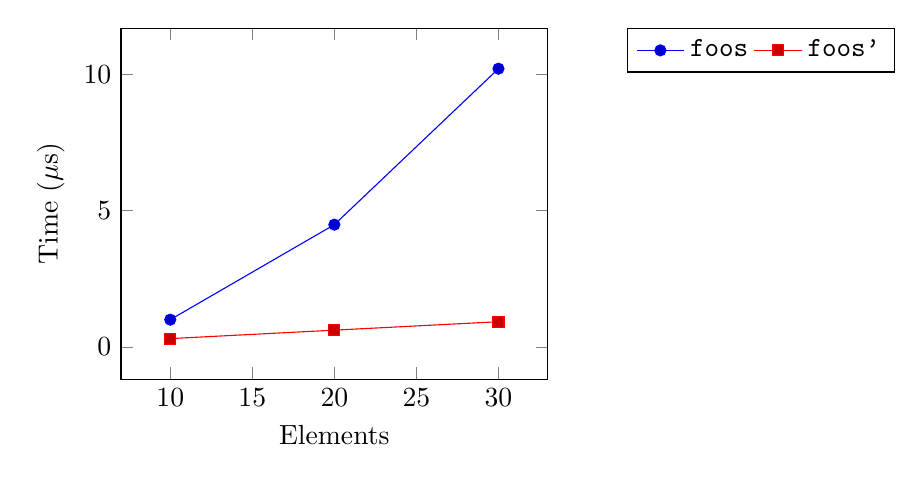
\begin{tikzpicture} \begin{axis}
		[
		legend style={at={(1.5,1)},
			anchor=north,legend columns=-1},
		enlargelimits=0.15,
		ylabel=Time ($\mu$s),
		xlabel=Elements
		]
		\addplot+ [
		sharp plot,
		] coordinates {(10,0.994) (20,4.48)
			(30,10.2)};
		\addplot+ [
		sharp plot,
		] coordinates {(10,0.300) (20,0.610) 
			(30,0.919)};
		\legend{\texttt{foos},\texttt{foos'}}
		\end{axis}
		\end{tikzpicture}
	\end{center}
\end{fancyfig}

You also saw that the following definition for the infinite list of Fibonacci numbers can be implemented elegantly and efficiently as the following in Haskell:
\begin{minted}{haskell}
fibs :: [Integer]
fibs = 1 : 1 : zipWith (+) fibs (tail fibs)
\end{minted}
The infinite list represented by \haskellIn{fibs} can be generated in linear time for the number of elements requested. This is possible because \haskellIn{fibs} is transformed into the following:
\begin{minted}{haskell}
fibs :: [Integer]
fibs = let xs = tail fibs 
           ys = zipWith (+) fibs xs
           zs = 1 : ys
       in 1 : zs
\end{minted}
All closures involved in this definition can be updated with their results. Therefore, \haskellIn{fibs} refers to a cons cell (a kind of closure) where the head is \haskellIn{1} and the closure pointed to by \texttt{\small zs} is the tail. The closure represented by \texttt{\small zs} is also a cons cell where the head is \haskellIn{1} and the tail is pointed to by \texttt{\small ys}. The closure represented by \texttt{\small ys} will be updated with the result of \haskellIn{zipWith (+) fibs xs} when more than two elements are requested from \haskellIn{fibs}, \emph{i.e.} the tail of \texttt{\small zs} is inspected by a \haskellIn{case}-expression somewhere. The \haskellIn{zipWith} function, in turn, allocates more closures when called, thus recursively adding more cons cells as needed.

However, not all closures can be updated. Suppose we want to generalise the definition of \haskellIn{fibs} to sequences with arbitrary seed values \texttt{\small x} and \texttt{\small y}:
\begin{minted}{haskell}
foos :: Integer -> Integer -> [Integer]
foos x y = x : y : zipWith (+) (foos x y) (tail (foos x y))
\end{minted}
This will be exponentially slow, because Haskell will not update the closure for \haskellIn{foos} with the list that is being generated. As a result, every call to \haskellIn{foos x y} will result in the list being generated from the beginning. This makes sense, because \haskellIn{foos} is parametrised over \texttt{\small x} and \texttt{\small y} and it would be wrong to update the closure for \haskellIn{foos} with the list generated for some specific \texttt{\small x} and \texttt{\small y}. 

\taskLine

\task[task:arbitrary-sequence]{Implement \haskellIn{foos'} to produce the same sequence as \haskellIn{foos}, but in linear time. \emph{Hint}: you need to find a way to allocate a closure which is specific to some \texttt{\small x} and \texttt{\small y} and can be updated.}

\task[task:lazy-bench]{You can run \bashIn{stack bench} to compare the time complexities of \haskellIn{foos} and \haskellIn{foos'}. If you have done everything right, you should see a bar graph with similar growth as the graph shown in \Cref{fig:foos-complexity} in the \texttt{\small benchmark.html} file which is generated by \bashIn{stack bench}.}

\taskLine